%%%%%%%%%%%%%%%%%%%%%%%%%%%%%%%%%%%%%%%%%
% Short Sectioned Assignment
% LaTeX Template
% Version 1.0 (5/5/12)
%
% This template has been downloaded from:
% http://www.LaTeXTemplates.com
%
% Original author:
% Frits Wenneker (http://www.howtotex.com)
%
% License:
% CC BY-NC-SA 3.0 (http://creativecommons.org/licenses/by-nc-sa/3.0/)
%
%%%%%%%%%%%%%%%%%%%%%%%%%%%%%%%%%%%%%%%%%

%----------------------------------------------------------------------------------------
%	PACKAGES AND OTHER DOCUMENT CONFIGURATIONS
%----------------------------------------------------------------------------------------

\documentclass[paper=a4, fontsize=11pt]{scrartcl} % A4 paper and 11pt font size

\usepackage[T1]{fontenc} % Use 8-bit encoding that has 256 glyphs
\usepackage{fourier} % Use the Adobe Utopia font for the document - comment this line to return to the LaTeX default
\usepackage[english]{babel} % English language/hyphenation
\usepackage{amsmath,amsfonts,amsthm} % Math packages

\usepackage{lipsum} % Used for inserting dummy 'Lorem ipsum' text into the template

\usepackage{enumitem}
\usepackage{mathtools}
\DeclarePairedDelimiter\ceil{\lceil}{\rceil}
\DeclarePairedDelimiter\floor{\lfloor}{\rfloor}
\usepackage{graphicx}
\usepackage{subfig}
\usepackage{listings}

\usepackage{sectsty} % Allows customizing section commands
\allsectionsfont{\centering \normalfont\scshape} % Make all sections centered, the default font and small caps

\usepackage{fancyhdr} % Custom headers and footers
\pagestyle{fancyplain} % Makes all pages in the document conform to the custom headers and footers
\fancyhead{} % No page header - if you want one, create it in the same way as the footers below
\fancyfoot[L]{} % Empty left footer
\fancyfoot[C]{} % Empty center footer
\fancyfoot[R]{\thepage} % Page numbering for right footer
\renewcommand{\headrulewidth}{0pt} % Remove header underlines
\renewcommand{\footrulewidth}{0pt} % Remove footer underlines
\setlength{\headheight}{13.6pt} % Customize the height of the header

\numberwithin{equation}{section} % Number equations within sections (i.e. 1.1, 1.2, 2.1, 2.2 instead of 1, 2, 3, 4)
\numberwithin{figure}{section} % Number figures within sections (i.e. 1.1, 1.2, 2.1, 2.2 instead of 1, 2, 3, 4)
\numberwithin{table}{section} % Number tables within sections (i.e. 1.1, 1.2, 2.1, 2.2 instead of 1, 2, 3, 4)

\setlength\parindent{0pt} % Removes all indentation from paragraphs - comment this line for an assignment with lots of text

%----------------------------------------------------------------------------------------
%	TITLE SECTION
%----------------------------------------------------------------------------------------

\newcommand{\horrule}[1]{\rule{\linewidth}{#1}} % Create horizontal rule command with 1 argument of height

\title{	
\normalfont \normalsize 
\textsc{University of Toronto, Department of ECE} \\ [25pt] % Your university, school and/or department name(s)
\horrule{0.5pt} \\[0.4cm] % Thin top horizontal rule
\huge ECE1762 - Homework 1 \\ % The assignment title
\horrule{2pt} \\[0.5cm] % Thick bottom horizontal rule
}

\author{Xinyun Lv(1001091178), Yang Wang(1001319227)} % Your name

\date{\normalsize\today} % Today's date or a custom date

\begin{document}

\maketitle % Print the title

%----------------------------------------------------------------------------------------
%	PROBLEM 1
%----------------------------------------------------------------------------------------

\section{Problem I}
Sort the following functions from asymptotically smallest to asymptotically largest.

\begin{center}
	$ 2^{log_{10}{n}} \quad log_{lg{n}}{n} \quad  lg(nlog{n})  \quad  n \quad (\sqrt{2})^{lg{n}} \quad (lglgn)^{lglgn} $
\end{center}


%----------------------------------------------------------------------------------------
%	PROBLEM 2
%----------------------------------------------------------------------------------------
%----------------------------------------------------------------------------------------
\section{Problem II}
Show that any sequence of $n^3 + 1$ numbers contains either
\begin{itemize}
	\item a strictly-increasing subsequence of length $n + 1$.
	\item a strictly-decreasing subsequence of length $n + 1$, or
	\item $n + 1$ elements with the same value.
\end{itemize}
\textbf{Proof:} \\
 Let $a_1, a_2, ..., a_{n^3 + 1}$ be a sequence of $n^3 + 1$ distinct real numbers. Let $f(n)$ be a function such that $ f(a_k) = (i_k, d_k, s_k) $ with $i_k$ being the length of the longest increasing subsequence starting at $a_k$ and $d_k$ being the length of the longest decreasing subsequence starting at $a_k$ and $s_k$ being the lenght of longest identical subsequence starting at $a_k$. \\
 \\
Suppose that the longest length of $i_k$, $d_k$ and $s_k$ is $n$. Then each $i_k$, $d_k$ and $s_k$ must between 1 and $n$\\
\\
This means there are $n^3$ possible $f(a_k) = (i_k, d_k, s_k)$. Since $k$ ranges from 1 to $n^3 + 1$, by the PHP theorem at least two of the $f(a_k)$ must contain the same values.\\
\\
This meas there must exist s < t such that $f(a_s) = f(a_t)$. So we have $i_s = i_t$, $d_s = d_t$ and $s_s = s_t$.\\
we have 3 cases:\\
\begin{itemize}
	\item if $a_s < a_t$ then $a_s$ could be added to the first of increasing sequence begin with $a_t$, which means $ i_s \ne i_t $. - a contradiction
	\item if $a_s > a_t$ then $a_s$ could be added to the first of decreasing sequence begin with $a_t$, which means $ d_s \ne d_t $. - a contradiction
	\item if $a_s = a_t$ then $a_s$ could be added to the identical sequence begin with $a_t$, which means $ s_s \ne s_t $. - a contradiction
\end{itemize}

Therefore, there must be an increasing, decreasing or identical subsequence of length $n+1$.

%----------------------------------------------------------------------------------------
%	PROBLEM 3
%----------------------------------------------------------------------------------------
%----------------------------------------------------------------------------------------
\section{Problem III}
 Solve the following recurrences. State tight asymptotic bounds for each function in the form $\Theta(f(n))$ for some recognizable function $f(n)$. Prove your answer. Assume reasonable but nontrivial base cases if none are supplied.

\begin{enumerate}[label=(\alph*)]
	\item $A(n)=2A(n/4)+nloglogn$
	\item $B(n) = B(n/2) + log n$
	\item $C(n)=3C(n/2)+nlogn$
	\item $F(n)=F(\floor*{logn})+logn$
\end{enumerate}
%----------------------------------------------------------------------------------------
%	PROBLEM 4
%----------------------------------------------------------------------------------------
%----------------------------------------------------------------------------------------
\section{Problem IV}
$m$ balls are thrown into $n$ bins (independently) so that each ball is equally likely to fall into any of the bins. Estimate as precisely as you can the smallest number $m$ (as a function of $n$) so that the probability of all balls falling into different bins is smaller than $\frac{1}{n^{c}}$, for a fixed constant $c>0$.\\
\textbf{Proof:}\\
Suppose that $x$: all balls falling into different bins
\begin{align*}
Pr(x) &= \frac{P(n, m)}{n^m}\\
&= \frac{n(n-1)(n-2)...(n-m+1)}{n^m}\\
&= \frac{(n-1)(n-2)...(n-m+1)}{n^{m - 1}}\\
&= \frac{\prod_{i=1}^{i=m-1}n - i}{n^{m - 1}}\\
&\leq \frac{(n-1)^{m-1}}{n^{m - 1}}\\
&= (1 - \frac{1}{n})^{m - 1}
\end{align*}
Since,
$$ 1 - \beta \leq e^{-\beta} $$
we have
$$ (1 - \frac{1}{n})^{m - 1} \leq e^{-\frac{m-1}{n}} $$
if 
$$ e^{-\frac{m-1}{n}} \leq \frac{1}{n^c} $$
then
$$ e^{\frac{m-1}{n}} \geq n^c$$
Apply $ln()$ on both sides,
$$ \frac{m-1}{n} \geq clnn $$
then we have,
$$ m - 1 \geq cnlnn $$
Therefore,
$$ m \geq cnlnn + 1$$

%----------------------------------------------------------------------------------------
%	PROBLEM 5
%----------------------------------------------------------------------------------------
%----------------------------------------------------------------------------------------
\section{Problem V}
Give a combinatorial argument to prove that
$$ \sum_{i=0}^{n}\dbinom{n}{i}2^{i} = 3^n $$

\textbf{Solution:} \\
\begin{figure}[h]
\centering
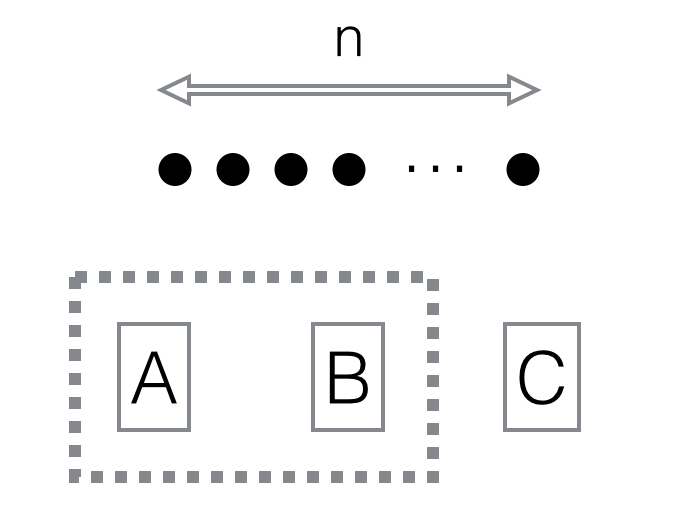
\includegraphics[scale=0.25]{p5img}
\caption{Problem 5}
\label{fig:p5}
\end{figure}\\

As shown in Figure \ref{fig:p5}, $n$ balls are thrown into 3 bins name A, B and C. The number of ways for $n$ balls falling into 3 bins is $3^n$ \\
\\
Also, the number of ways for $n$ balls not falling into bin C for $i$ times is: $\dbinom{n}{i} 2^{i}$. Then , we have the possibility of $n$ balls not falling into bin C for i times is:
$$\frac{\dbinom{n}{i} 2^{i}}{3^n}$$
As $0 \leq i \leq n$, the sum of possibilities of $\frac{\dbinom{n}{i} 2^{i}}{3^n}$ from $i = 0$ to $i = n$ should be 1, as it contains all the possible results for throwing $n$ balls into 3 bins.\\
Therefore,
$$ \frac{\sum_{i=0}^{n}\dbinom{n}{i}2^{i}}{3^n} = 1$$
$$\sum_{i=0}^{n}\dbinom{n}{i}2^{i} = 3^n$$
%----------------------------------------------------------------------------------------
%	PROBLEM 6
%----------------------------------------------------------------------------------------
%----------------------------------------------------------------------------------------
\section{Problem VI}
Consider a light ray entering two adjacent planes of glass on a table. At any meeting surface (between the two planes of glass, or between the top glass and the air) the light may either reflect (bounce) or continue straight through (refract). In the example below, the light ray bounces 7 times before it leaves the glass plane. The light always reflects between the bottom glass and the table. How many different paths can a light ray take if it bounces $n$ times before it leaves the top glass plane? Give a recurrence relation to answer this question.\\\\
\textbf{Solution:} \\
According to the Figure of problem, we can notice that for any $n$ is even, $F(n) = 0$.\\
If $n$ is an odd, we will have following 5 basic paths below for the last two reflections before it leaves table:\\
\begin{figure}[h]
	\centering
	\subfloat[Subfigure 1 list of figures text][Path case 1]{
		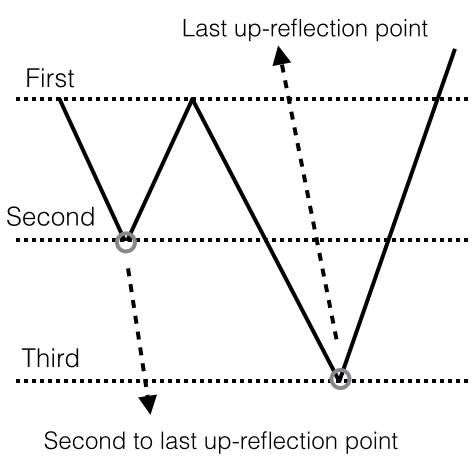
\includegraphics[width=0.2\textwidth]{path1}
		\label{fig:p6subfig1}}
	\subfloat[Subfigure 2 list of figures text][Path case 2]{
		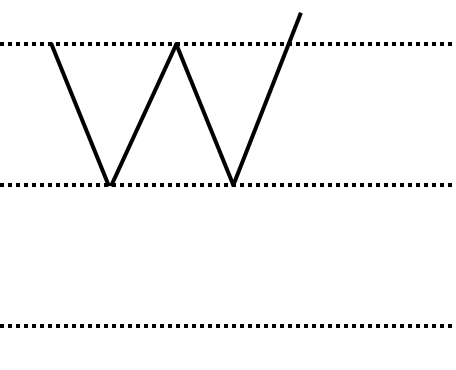
\includegraphics[width=0.2\textwidth]{path2}
		\label{fig:p6subfig2}}\\
	\subfloat[Subfigure 3 list of figures text][Path case 3]{
		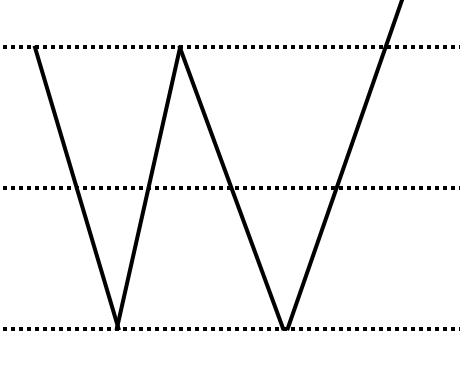
\includegraphics[width=0.2\textwidth]{path3}
		\label{fig:p6subfig3}}
	\subfloat[Subfigure 4 list of figures text][Path case 4]{
		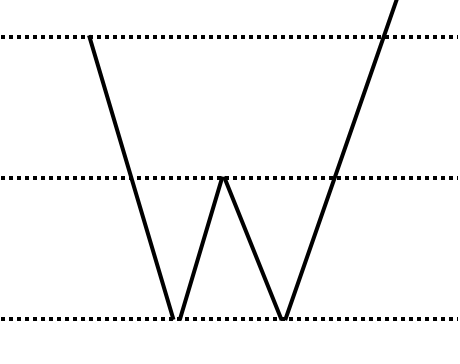
\includegraphics[width=0.2\textwidth]{path4}
		\label{fig:p6subfig4}}
	\subfloat[Subfigure 5 list of figures text][Path case 5]{
		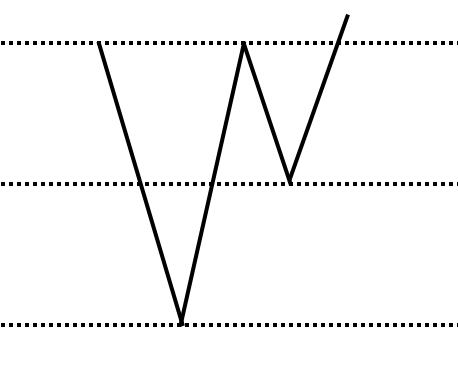
\includegraphics[width=0.2\textwidth]{path5}
		\label{fig:p6subfig5}}
	\caption{5 basic paths for the last two reflections}
	\label{fig:p6fig}	
\end{figure}\\
As shown in Figure \ref{fig:p6fig}, we can note that if the second to last up-reflection point is on the second level from the top, there are two kinds possible paths to leave table as shown in Figure \ref{fig:p6subfig1} and Figure \ref{fig:p6subfig2}. We can also notice that if the second to last up-reflection point is on the second level from top, the last up-reflection point will have $\frac{1}{2}$ possiblity to be on the second level from top as shown in Figure \ref{fig:p6subfig1} and $\frac{1}{2}$ possiblity to be on the third level from top as shown in Figure \ref{fig:p6subfig2}. However, if the second to last up-reflection point is on the third level from top, there are three kinds of possible paths to leave table as shown in Figure \ref{fig:p6subfig3}, Figure \ref{fig:p6subfig4} and Figure \ref{fig:p6subfig5}. Similarly, we could note that if the second to last up-reflection point is on the third level from top, the last up-reflection point will have $\frac{1}{3}$ possiblity to be on the second level from top as shown in Figure \ref{fig:p6subfig5} and $\frac{2}{3}$ possiblity to be on the third level from top as shown in Figure \ref{fig:p6subfig3} as well as Figure \ref{fig:p6subfig4}.\\\\

Based on the discussion above, we could analysis possible paths for $F(n)$. To get the recurrence relation of $F(n)$, we need to analyze $F(n - 2)$ and $F(n - 4)$. \\\\
we could assume that there are $p_1$ numbers of paths in $F(n - 4)$ whose last up-reflection point is on the third level from top and $p_2$ numbers of paths in $F(n - 4)$ whose last up-reflection point is on the second level from top. Thus, we have:
$$ F(n - 4) = p_1 + p_2 $$
Also, according to the disscussion and Figure \ref{fig:p6fig} above, we have:
$$ F(n - 2) = 3p_1 + 2p_2 $$
\begin{align*}
F(n) &= 3[(3p_1)\cdot \frac{2}{3} + (2p_2)\cdot \frac{1}{2}] + [(3p_1)\cdot \frac{1}{3} + (2p_2)\cdot \frac{1}{2}]\\
&= 8p_1 + 5p_2
\end{align*}
Based one this three equations, we can get $p_1 = F(n - 2) - 2F(n - 4)$, $p_2 = 3F(n - 4) - F(n - 2)$.
Thus, we have
\begin{align*}
F(n) = 
\begin{cases}
0 & n $ is even$\\
3F(n - 2) - F(n - 4) & n $ is odd$
\end{cases}
\end{align*}




\end{document}